%22
\subsection{Új elem beillesztése adott elem után}
\begin{frame}
  \begin{center}
    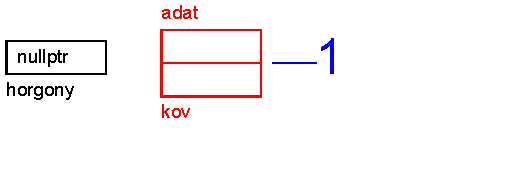
\includegraphics[scale=0.6]{lista1/list1-01.pdf}
  \end{center}
  \vspace{-.2cm}
  \meret{7}
  \begin{exampleblock}{\textattachfile{Lista1.cpp}{Lista1.cpp}}
    \vspace{-.2cm}
    \lstinputlisting[style=cpp,linerange={5-18},numbers=left,firstnumber=5]{Lista1.cpp}
    \vspace{-.2cm}
  \end{exampleblock}
\end{frame}

%23
\begin{frame}
  \begin{center}
    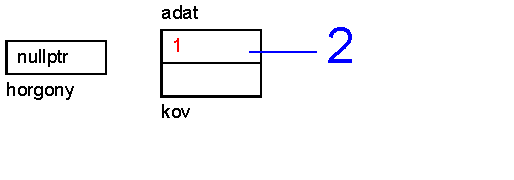
\includegraphics[scale=0.6]{lista1/list1-02.pdf}
  \end{center}
  \vspace{-.2cm}
  \meret{7}
  \begin{exampleblock}{\textattachfile{Lista1.cpp}{Lista1.cpp}}
    \vspace{-.2cm}
    \lstinputlisting[style=cpp,linerange={5-18},numbers=left,firstnumber=5]{Lista1.cpp}
    \vspace{-.2cm}
  \end{exampleblock}
\end{frame}

%24
\begin{frame}
  \begin{center}
    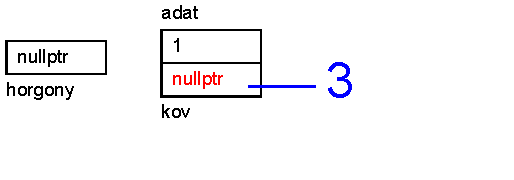
\includegraphics[scale=0.6]{lista1/list1-03.pdf}
  \end{center}
  \vspace{-.2cm}
  \meret{7}
  \begin{exampleblock}{\textattachfile{Lista1.cpp}{Lista1.cpp}}
    \vspace{-.2cm}
    \lstinputlisting[style=cpp,linerange={5-18},numbers=left,firstnumber=5]{Lista1.cpp}
    \vspace{-.2cm}
  \end{exampleblock}
\end{frame}

%25
\begin{frame}
  \begin{center}
    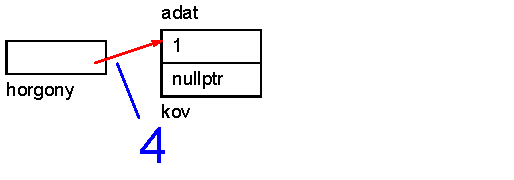
\includegraphics[scale=0.6]{lista1/list1-04.pdf}
  \end{center}
  \vspace{-.2cm}
  \meret{7}
  \begin{exampleblock}{\textattachfile{listaTeszt1.cpp}{listaTeszt1.cpp}}
    \vspace{-.2cm}
    \lstinputlisting[style=cpp,linerange={6-18},numbers=left,firstnumber=6]{listaTeszt1.cpp}
    \vspace{-.2cm}
  \end{exampleblock}
\end{frame}

%26
\begin{frame}
  \begin{center}
    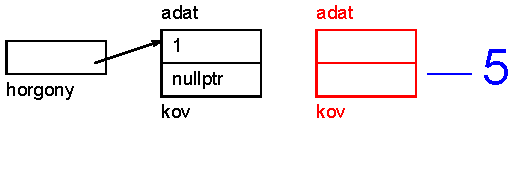
\includegraphics[scale=0.6]{lista1/list1-05.pdf}
  \end{center}
  \vspace{-.2cm}
  \meret{7}
  \begin{exampleblock}{\textattachfile{Lista1.cpp}{Lista1.cpp}}
    \vspace{-.2cm}
    \lstinputlisting[style=cpp,linerange={5-18},numbers=left,firstnumber=5]{Lista1.cpp}
    \vspace{-.2cm}
  \end{exampleblock}
\end{frame}

%27
\begin{frame}
  \begin{center}
    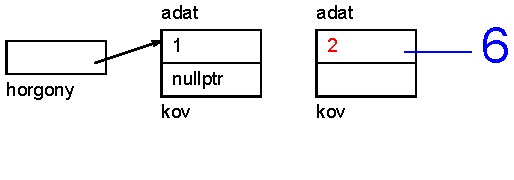
\includegraphics[scale=0.6]{lista1/list1-06.pdf}
  \end{center}
  \vspace{-.2cm}
  \meret{7}
  \begin{exampleblock}{\textattachfile{Lista1.cpp}{Lista1.cpp}}
    \vspace{-.2cm}
    \lstinputlisting[style=cpp,linerange={5-18},numbers=left,firstnumber=5]{Lista1.cpp}
    \vspace{-.2cm}
  \end{exampleblock}
\end{frame}

%28
\begin{frame}
  \begin{center}
    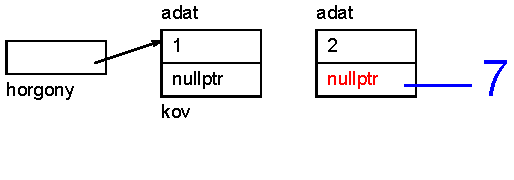
\includegraphics[scale=0.6]{lista1/list1-07.pdf}
  \end{center}
  \vspace{-.2cm}
  \meret{7}
  \begin{exampleblock}{\textattachfile{Lista1.cpp}{Lista1.cpp}}
    \vspace{-.2cm}
    \lstinputlisting[style=cpp,linerange={5-18},numbers=left,firstnumber=5]{Lista1.cpp}
    \vspace{-.2cm}
  \end{exampleblock}
\end{frame}

%29
\begin{frame}
  \begin{center}
    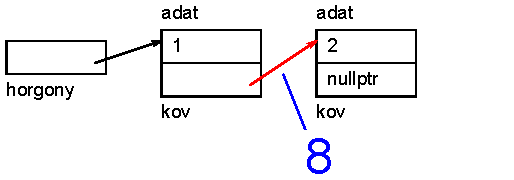
\includegraphics[scale=0.6]{lista1/list1-08.pdf}
  \end{center}
  \vspace{-.2cm}
  \meret{7}
  \begin{exampleblock}{\textattachfile{listaTeszt1.cpp}{listaTeszt1.cpp}}
    \vspace{-.2cm}
    \lstinputlisting[style=cpp,linerange={6-18},numbers=left,firstnumber=6]{listaTeszt1.cpp}
    \vspace{-.2cm}
  \end{exampleblock}
\end{frame}